\newpage
\section{Introduction}
\subsection{\small General Formulation of the Optimization Problem}

Let $x$ be an n-dimensional real vector
\begin{align*}
    \bm{x}=\left( x^{(1)}, \dots, x^{(n)} \right)^T\in \mathbb{R}^n
\end{align*}
and $f_0(x),\dots,f_m(x)$ be some \textbf{real-valued} function defined  on a set $S\subseteq \mathbb{R}^n$. We consider different variants of the following general minimization problem:
\begin{align}
    \notag &\min f_0(\bm x)\\
    \label{P1} \st &f_j(\bm x) \& 0, j=1\dots m\\
    \notag  &\bm{x} \in S
\end{align}
where the sign $\&$ can be $\le, \ge$ or $=$. 

\& 表示受约束. 可用$\le$ 表示$\ge$, 然后用 $\le, \ge$ 表示 $=$. 

We call $f_0(x)$ the \textbf{objective function} (目标函数) of our problem, the vector function
\begin{align*}
    f(\bm x)=\left( f_1(x),\dots,f_m(x) \right)^T
\end{align*}
is called the vector of \textbf{functional constraints} (泛函约束), the set $S$ is the \textbf{basic feasible set} (基本可行集), and the set
\begin{align*}
    Q=\{ \bm x \in S\ |\ f_j(\bm x)\le 0,j=1,\dots,m \}
\end{align*}
is the \textbf{(entire) feasible set} (完整可行集) of problem \ref{P1}. It's just a convention to consider minimization problems. 

\subsubsection{Natural Classification}
There exists a natural classification of the types of minimization problems:
\begin{itemize}\small
    \item Constrained problems (带约束问题): $Q\subset \mathbb{R}^n$
    \item Unconstrained problems (无约束问题): $Q\equiv \mathbb{R}^n$
    \item smooth problems (光滑问题): all $f_j(x)$ are differentiable
    \item nonsmooth problems: some $f_k(x)$ are non-differentiable
    \item linearly constrained problems: the functional constraints are affine (仿射) like
    \begin{align*}
        f_j(\bm{x})=\sum_{i=1}^n a_j^{(i)}\bm x^{(i)}+b_j\equiv\braket{a_j,\bm x}+b_j,\ j=1,\dots,m
    \end{align*}
    \begin{itemize}
        \item linear optimization problem: $f_0(\cdot)$ is also affine
        \item quadratic optimization problem: $f_0(\cdot)$ is quadratic
        \item quadratically constrained problem: all the function $f_0(\cdot),\dots,f_m(\cdot)$ are quadratic
    \end{itemize}
\end{itemize}

\subsubsection{Classification based on the properties of feasible set}
There is also a classification based on properties of the feasible set. 
\begin{itemize}
    \item Problem \ref{P1} is called \textbf{feasible}, if $Q\ne \emptyset$
    \item Problem \ref{P1} is called \textbf{strictly feasible}, if there exists an $\bm x \in $ int $Q$ such taht $f_j(\bm x)<0$ (or $>0$) for all inequality constraints and $f_j(\bm x)=0$ for all equality constraints (Slater condition)
\end{itemize}
int $Q$ 表示不包含 边界点的 $Q$.

\subsubsection{Different Types of Solution}
Finally, we distinguish different types of solution to \ref{P1}:
\begin{itemize}
    \item $\bm x^*$ is called the \textbf{global optimal solution} to \ref{P1} if $f_0(\bm x^*)\le f_0(x)$ for all $x\in Q$. In this case, $f_0(\bm x^*)$ is called the (global) \textbf{optimal value} of the problem. ($\bm x^*=\arg \min \cdots$, 是个集合)
    \item $\bm x^*$ is called a  \textbf{local optimal solution} to \ref{P1} if $\exists\delta$, for all $\bm x\in NBR(\bm x^*, \delta)\cap Q$ ($NBR$ means Neighborhood), we have 
    \begin{align*}
        f_0(\bm x^*)\le f_0(\bm x)
    \end{align*}
\end{itemize}

\subsubsection{Example}
\paragraph{Example 1} Let $\bm x^{(1)},\dots,\bm x^{(n)}$ be our \textbf{design variables}. Then we can fix some functional characteristics of our decision vector $\bm x:f_0(\bm x),\dots,f_m(\bm x)$. For example, we can consider a price of the project, amount of required resources, reliability of the system, etc. We fix the most important characteristics, $f_0(\bm x)$, as our objective. For all others, we impose some bounds: $a_j\le f_j(\bm x)\le b_j$. Thus, we come to the problem:
\begin{align*}
    &\min f_0(\bm x)\\
    \st &a_j\le f_j(\bm x) \le b_j, j=1\dots m\\
    &\bm{x} \in S
\end{align*}
where $S$ stands for the \textbf{structural} constraints like non-negativity, boundedness of some variables, etc. 

\paragraph{Example 2} Let our initial problem be as follow:
\begin{align}
    \label{P2} \text{Find } \bm x \in \mathbb{R}^n \text{ such that }f_j(\bm x)=a_j, j=1,\dots,m
\end{align}
Then we consider the problem
\begin{align*}
    \min_{\bm x}\sum_{j=1}^m(f_j(\bm x)-a_j)^2
\end{align*}
perhaps evne with some additional constraints on $\bm x$.  If the optimal value of the latter problem is zero, we conclude that our initial problem \ref{P2} has a solution.

\paragraph{Example 3} Sometimes our decision variables $\bm x^{(1)},\dots,\bm x^{(n)}$ must be integers. This can be described by the following constraint:
\begin{align*}
    \sin(\pi \bm x^{(i)})=0, i=1,\dots,n
\end{align*}
Thus, we can also treat integer optimization problems:
\begin{align*}
    &\min f_0(\bm x)\\
    \st & a_j \le f_j(\bm x) \le b_j, j=1,\dots,m\\
    &\bm x\in S\\
    &\sin(\pi \bm x^{(i)})=0, i=1,\dots,n
\end{align*}

\subsection{\small Interplay of Optimization and Machine Learning}
\subsubsection{The Machine Learning (Supervised) Paradigm}
Consider the following \textbf{spaces}: a space of \textit{example} $\mathcal{X}$, a space of \textbf{labels} $\mathcal{Y}$, and a space of \textit{hypothesis} $\mathcal{H}$ that contains functions mapping $\mathcal{X}$ to $\mathcal{Y}$. Also consider a \textbf{loss} function $L: \mathcal{Y}\times \mathcal{Y}\to \mathbb{R}$ and a \textbf{probability measure} $P$ over the space $\mathcal{X} \times \mathcal{Y}$. 

\begin{definition}
    For any hypothesis $h\in \mathcal{H}$, we define the risk of $h$ with respect to $L$ and $P$ to be:
    \begin{align*}
        \mathcal{L}_P(h)=E_P(L(h(\bm X), Y)),\text{ with }(\bm X, Y)\sim P
    \end{align*}

    The general problem of machine learning can be then cast as finding the hypothesis $h\in\mathcal{H}$ that  solves the following optimization problems:
    \begin{align*}
        \min_{h\in \mathcal{H}}\mathcal{L}_P (h)
    \end{align*}
\end{definition}

\subsubsection{Empirical Risk Minimization}
The practical way is to solve an \textit{empirical risk minimization} problem. That is,
\begin{align*}
    \min_{h\in \mathcal{H}}\sum_{i=1}^m L(h(\bm x_i), y_i)=\min_\theta \sum_{i=1}^m L(h_\theta(\bm x_i), y_i)
\end{align*}
since we do not know the $P$ exactly. That is
\begin{align*}
    \theta_*=\argmin_\theta \sum_{i=1}^m L(h_\theta(\bm x_i), y_i)
\end{align*}

\begin{itemize}
    \item Classification: the output variable takes \textbf{class labels}. Especially, for \textbf{binary classification}, $y_i\in\{1,-1\}$. 
    \item Regression: the output variable takes \textbf{continuous values}. That is $y_i \in\mathbb{R}$. 
\end{itemize}

\subsubsection{Classification: \texorpdfstring{The $0\sim 1$ Loss}.} 
By using the $0\sim1$ \textit{loss}, we can rewrite the objective function as:
\begin{align*}
    \sum_{i=1}^m \bm 1_{\mathrm{sign}(h(\bm x_i))\ne y_i}=\sum_{i=1}^m\bm 1_{y_ih(\bm x_i)<0}
\end{align*}
where $\bm 1_z$ is just the indicator function, that is
\begin{align*}
    \bm 1_z=\left\{ \begin{array}{ll}
        1 & z\text{ is true}\\
        0 & \text{otherwise}
    \end{array} \right.
\end{align*}
and $\mathrm{sign}(x)$ is sign function,
\begin{align*}
    \mathrm{sign}(x)=\left\{ \begin{array}{ll}
        1 & x>0\\
        0 & x=0\\
        -1 & x<0
    \end{array} \right.
\end{align*}

In fact, this problem is \textbf{NP-hard} so it's pointless to try to minimize this function. 

\paragraph{The Surrogate of The \texorpdfstring{$0\sim 1$}. Loss}To deal with this problem, we can introduce some \textit{surrogate}. 

\begin{figure}[!htb]
    \centering
    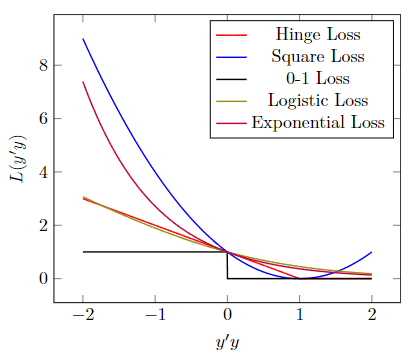
\includegraphics[width=0.309\textwidth]{pic/Opt1/Surrogate.png}
    \caption{The Surrogate of The $0\sim 1$ Loss}
\end{figure}

Some common loss function 
\begin{itemize}
    \item hinge loss or margin loss 
    \begin{align*}
        \phi_h(y,y')=\max(0,1-y'y)
    \end{align*}
    \item Square loss: 
    \begin{align*}
        \phi_s(y,y')=(1-yy')^2
    \end{align*}
    \item Logistic loss: 
    \begin{align*}
        \phi_l(y,y')=\frac{1}{\ln 2}\ln(1+e^{-yy'})
    \end{align*}
    \item Exponential loss: 
    \begin{align*}
        \phi_e(y,y')=e^{-yy'}
    \end{align*}
    \item Cross entropy loss: 
    \begin{align*}
        \phi_c(y,y')=-t\ln(y')-(1-t)\ln(1-y')
    \end{align*}
    where $t=\frac{(1+y)}{2}$
\end{itemize}

\subsubsection{Maximum Likelihood Estimation View}
Let's say, we have a likelihood function $P(\bm X, Y|\theta)$. Then the MLE for $\theta$, the parameter we want to infer, is 
\begin{align*}
    \theta_{MLE}&=\argmax_\theta P(\bm X, Y|\theta)\\
    &=\argmax_\theta \log P(\bm X, Y|\theta)\\
    &=\argmax_\theta \log \prod_i P(x_i, y_i|\theta)\\
    &=\argmax_\theta \sum_{i=1}^n \log P(x_i, y_i|\theta)
\end{align*}
For case that $P(x_i, y_i|\theta)\sim \exp(-L(h_\theta(\bm x_i), y_i))$ ($\sim$ 表示成比例), we have
\begin{align*}
    \theta_{MLE}=\argmin_\theta \sum_{i=1}^n L(h_\theta(\bm x_i), y_i)
\end{align*}

\subsubsection{Maximum A posteriori Estimation View}
If we replace the likelihood in the MLE formula above with the posterior, we get:
\begin{align*}
    \theta_{MAP}&=\argmax_\theta P(\bm X, Y|\theta)P(\theta)\\
    &=\argmax_\theta\log\{ P(\theta)P(\bm X, Y|\theta) \}\\
    &=\argmax_\theta\log \left\{ P(\theta)\prod_i P(\bm x_i, y_i|\theta) \right\}\\
    &=\argmax_\theta\left\{ \log P(\theta)+\sum_{i=1}^n \log P(\bm x_i, y_i|\theta)\right\}
\end{align*}
For case that $P(x_i, y_i|\theta)\sim \exp(-L(h_\theta(\bm x_i), y_i))$ and $P(\theta)\sim \exp(-\lambda\|\theta\|_2^2)$, we have
\begin{align*}
    \theta_{MAP}=\argmax_\theta\left\{ \sum_{i=1}^n L(h_\theta(\bm x_i), y_i)+\lambda \|\theta\|_2^2 \right\}
\end{align*}

$P(\theta)$ 作为先验, 推导出正则项. 正则化可以让函数凸性更好, 更容易找到最小值. 

\subsection{Performance of Numerical Methods}
\subsubsection{Method and Class of Problem}
% Consider a method for solving problem \ref{P1}: which does nothing except that $x^*=0$. For those which have the optimal solution exactly at the origin, the ``performance'' of this method is \textbf{unbeatable}. Also, this method doesn't work properly for any other problems. Hence, we can't speak about the best method for a particular problem $P$, but we can do so for a class of problems $\mathcal{F} \ni P$. (对一类问题)

% The performance of a method $\mathcal{M}$ on the whole class $\mathcal{P}$ can be natural measure of its efficiency. Consider the performance of $\mathcal{M}$ on a class $\mathcal{P}$. We should assume that the method $\mathcal{M}$ doesn't have complete information about a particular problem $\mathcal{P}$. 


% \begin{itemize}
%     \item \textbf{Model}: The konwn (to a numerical scheme) ``part'' of problem $\mathcal{P}$ is called the model of the problem. We denote the model by $\Sigma$. Usually the model consists of the formulation of the problem, description of classes of functional components, etc.  (已知的信息)
%     \item \textbf{Oracle}: We describe the process of collecting the specific information about $\mathcal{P}$ via the notion of an oracle. AN oracle $\mathcal{O}$ is just a unit which answers the successive questions of the methods.  (需要回答的问题, 需要给出的输出)
% \end{itemize}
% In general, each problem can be described by different models. Moreover, for each problem we can develop different types of oracles. 

考虑一种解决问题 \ref{P1} 的方法:除了$x^*=0$之外, 什么都不做. 对于那些在原点恰好有最优解的问题, 这种方法的``性能''是无法超越的. 然而, 这种方法对于其他任何问题都无法正常工作. 因此, 我们不能说某个特定问题$P$的最佳方法是什么, 但我们可以针对一类问题$\mathcal{F} \ni P$来讨论. 

一个方法$\mathcal{M}$在整个类别$\mathcal{P}$上的性能可以自然地衡量其效率. 考虑$\mathcal{M}$在类别$\mathcal{P}$上的性能. 我们应该假设方法$\mathcal{M}$并没有关于特定问题$\mathcal{P}$的完整信息. 

\begin{itemize}
    \item \textbf{Model}:已知(对数值方案)``部分''问题$\mathcal{P}$被称为问题的模型. 我们用$\Sigma$表示模型. 通常, 模型包括问题的表述、功能组件类别的描述等. 
    \item \textbf{Oracle}:我们通过预言的概念描述收集关于$\mathcal{P}$的特定信息的过程. 预言$\mathcal{O}$只是一个回答方法连续问题的单位. 
\end{itemize}
一般来说, 每个问题都可以用不同的模型来描述. 此外, 对于每个问题, 我们都可以开发出不同类型的预言. 

Let us fix $\Sigma$ and $\mathcal{O}$. In this case, it's natural to define the performance of $\mathcal{M}$ on $(\Sigma, \mathcal{O})$, as its performance on the worst $\mathcal{P}_w$ from $(\Sigma, \mathcal{O})$. Note that this $\mathcal{P}_w$ can be bad only fo $\mathcal{M}$. 
\begin{definition}
    The performance of $\mathcal{M}$ on $\mathcal{P}$ is the total amount of computational effort required by method $\mathcal{M}$ to solve the problem $\mathcal{P}$. 
\end{definition}
Solving the problem means finding an approximate solution on $\mathcal{P}$ with some accuracy $\epsilon>0$ (找逼近解就是解问题了). 

\subsubsection{General Iterative Scheme}
\begin{itemize}
    \item Input: Starting point $x_0$ and accuracy $\epsilon>0$
    \item Initialization: Set $k=0, I_{-1}=\emptyset$
\end{itemize}

Main Loop:
\begin{enumerate}
    \item Call oracle $\mathcal{O}$ at point $x_k$
    \item Update the information set: $I_k=I_{k-1}\cup (x_k, \mathcal{O}(x_k))$
    \item Apply the rules of method $\mathcal{M}$ to $I_k$ and generate a new point $x_{k+1}$
    \item Check criterion $\mathcal{T}_\epsilon$. If \textbf{yes} then form an output $\bar{\bm x}$. Otherwise set $k:=k+1$ and go to Step 1. 
\end{enumerate}

\subsubsection{Complexity}
In above scheme,  we can see two potentially expensive steps. The first one is Step 1, where we call the oracle. The second one is Step 3, where we form the new test point. Thus, we can introduce two measures of complexity of problem $\mathcal{P}$ for method $\mathcal{M}$:
\begin{itemize}
    \item Analytical Complexity: The number of calls of the oracle which is necessary to solve problem $\mathcal{P}$ up to accuracy $\epsilon$. 
    \item Arithmetical Complexity: The total number of arithmetic operations (including the work of both oracle and method ), which is necessary to solve problem $\mathcal{P}$ up to accuracy $\epsilon$. 
\end{itemize}
For a particular method $\mathcal{M}$ as applied to problem $\mathcal{P}$, arithmetical complexity can be easily obtained from the analytical complexity and complexity of the oracle.

\subsubsection{Oracle}
There is one standard assumption on the oracle which allows us to obtain the majority of results on analytical complexity for optimization schemes. This assumption, called the \textbf{Local Black Box Concept}, is listed in the following lines:
\begin{enumerate}
    \item The only information available for the numerical scheme is the answer of the oracle.
    \item The oracle is local: A small variation of the problem far enough from the test point $x$, which is compatible with the description of the problem class, does not change the answer at $x$
\end{enumerate}

The standard formulation \ref{P1} is called a functional model of optimization problems. Usually, for such models the standard assumptions are related to the level of smoothness of functional components. According to the degree of smoothness we can apply different types of oracle:
\begin{itemize}
    \item zero-order oracle: return $f(x)$
    \item first-order oracle: return $f(x)$ and gradient $\nabla f(x)$
    \item second-order oracle: return $f(x)$, gradient $\nabla f(x)$ and Hessian $\nabla^2 f(x)$
\end{itemize}

\subsection{Complexity Bounds for Global Optimization}
\subsubsection{N-dimensional Box Constraint Problem}
Consider the following problem:
\begin{align}
    \min_{x\in \mathbb{B}_n}f(x) \label{P4}
\end{align}
In our terminology, this is a constrained minimization problem with no functional constraints. The basic feasible set of this problem is $\mathbb{B}_n$, an n-dimensional box in $\mathbb{R}^n$:
\begin{align*}
    \mathbb{B}_n=\{ \bm x\in \mathbb{R}^n\ |\ 0\le \bm x^{(i)}\le 1,\ i=1,\dots,n \} ;
\end{align*}

\begin{figure}[!htb]
    \centering
    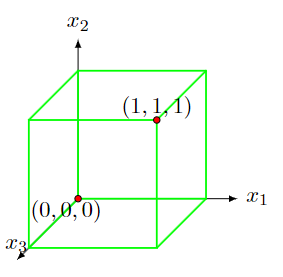
\includegraphics[width=0.22\textwidth]{pic/Opt1/N-d Box.png}
    \caption{N-dimensional Box Constraint Problem}
\end{figure}

Let us measure distances in $\mathbb{R}^n$ by the ${\ell}_\infty$:
\begin{align*}
    \|\bm x\|_\infty=\max_{1\le i\le n}|\bm x^{(i)}|
\end{align*}
Assume that, with respect to this norm, the objective function $f(\bm x):\mathbb{R}^n\to \mathbb{R}$ is \textbf{Lipschitz continuous} on $\mathbb{B}_n$:
\begin{align}
    |f(\bm x)-f(\bm y)|\le L\| \bm x-\bm y \|_\infty, \forall \bm x, \bm y\in \mathbb{B}_n \label{P5}
\end{align}
with some constant $L$ (\textbf{Lipschitz constant}).

\subsubsection{Uniform Grid Method}
Method $\mathcal{G}(p)$:
\begin{enumerate}
    \item Form $(p+1)^n$ points
    \begin{align*}
        \bm x_{(i_1,\dots,i_n)}=\left( \frac{i_1}{p}, \frac{i_2}{p},\dots,\frac{i_n}{p} \right)^T
    \end{align*}
    where $(i_1,\dots,i_n) \in \{ 0, \dots,p\}^n$.
    \item Among all points $\bm x_{(i_1,\dots,i_n)}$, find the point $\bar{\bm x}$ with the minimal value of the objective function.
    \item The pair $(\bar{\bm x}, f(\bar{\bm x}))$ is the output of the method.
\end{enumerate}
This method forms a \textbf{uniform grid} of the test points inside the box $\mathbb{B}_n$, computes the best value of the objective over this grid, and returns this value as an approximate solution to problem \ref{P4}. 
\begin{itemize}
    \item Zeroorder iterative method,
    \item Without any influence from the accumulated information on the sequence of test points.
\end{itemize}

\begin{theorem}\label{T5}
    Let $f^*$ be a global optimal value of problem \ref{P4}. Then
    \begin{align*}
        f(\bar{\bm x})-f^*\le \frac{L}{2p}
    \end{align*}
\end{theorem}

\begin{proof}
    For a multiindex $(i_1,i_2,\dots,i_n)$, let $\bm x_*$ be a global minimum of our problem, Then there exist coordinates $(i_1,i_2,\dots,i_n)$ such that
    \begin{align*}
        \bm x\equiv \bm x_{(i_1,i_2,\dots,i_n)}\le \bm x_* \le \bm x_{(i_1+1,i_2+1,\dots,i_n+1)}\equiv \bm y
    \end{align*}
    Note that
    \begin{align*}
        \bm y^{(i)}-\bm x^{(i)}=\frac{1}{p}
    \end{align*}
    for $i=1,\dots,n$ and 
    \begin{align*}
        \bm x_*^{(i)}\in [\bm x^{(i)},\bm y^{(i)}],i=1,\dots,n
    \end{align*}

    \begin{figure}[!htb]
        \centering
        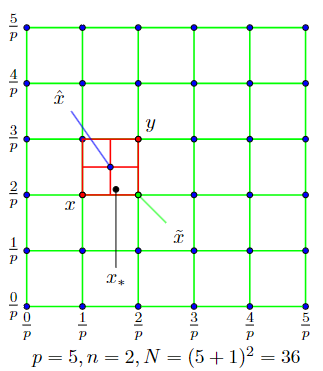
\includegraphics[width=0.22\textwidth]{pic/Opt1/Uniform Grid Method}
        \caption{Uniform Grid Method}
    \end{figure}
    Denote $\hat{\bm x}=(x+y)/2$. Let's form a point $\tilde{\bm x}$ as follows:
    \begin{align*}
        \tilde{\bm x}=\left\{ \begin{array}{ll}
            \bm y^{(i)} & \text{if }\bm x_*^{(i)}\ge \hat{\bm x}^{(i)}\\
            \bm x^{(i)} & \text{otherwise}
        \end{array} \right.
    \end{align*}
    It's clear that $|\tilde{\bm x}^{(i)}-\bm x_*^{(i)}|\le \frac{1}{2p}, i=1,\dots,n$. Therefore
    \begin{align*}
        \|\tilde{\bm x}-\bm x_*\|_\infty=\max_{1\le i\le n} |\tilde{\bm x}^{(i)}-\bm x_*^{(i)}|\le \frac{1}{2p}
    \end{align*}
    Since $\tilde{\bm x}$ belongs to our grid, we conclude that
    \begin{align*}
        f(\bar{\bm x})-f(\bm x_*)\le f(\tilde{\bm x})-f(\bm x_*)\le L\|\tilde{\bm x}-\bm x_*\|_\infty\le \frac{L}{2p}
    \end{align*}
\end{proof}


\subsubsection{Upper Complexity Bound}
Let us conclude with the definition of our problem class. We fix our goal as follows:
\begin{align}
    \text{Find }\bar{\bm x}\in \mathbb{B}_n:f(\bar{\bm x})-f^*\le \epsilon \label{P7}
\end{align}
Then we immediately get the following result.

\begin{corollary}
    The analytical complexity of problem class \ref{P4}, \ref{P5}, \ref{P7} for method $\mathcal{G}$ is at most
    \begin{align*}
        \mathcal{A}(\mathcal{G})=\left( \left\lfloor \frac{L}{2\epsilon} \right\rfloor +2 \right)^n
    \end{align*}
\end{corollary}

\begin{proof}
    Take $p=\left\lfloor \frac{L}{2\epsilon} \right\rfloor+1$. Then $p\ge \frac{L}{2\epsilon}$. and , in view of Theorem \ref{T5}, we have
    \begin{align*}
        f(\bar{\bm x})-f^*\le \frac{L}{2p}\le \epsilon
    \end{align*}
    Note that we construct $(p + 1)^n$ points.
\end{proof}

Remark:
\begin{itemize}
    \item Each point has an access to oracle, so the number of accessing is equal to the number of points.
    \item Thus, $\mathcal{A}(\mathcal{G})$ justifies an upper complexity bound for our problem class.
\end{itemize}

\subsubsection{Lower Complexity Bound}
% Two situations should be further explored:
% \begin{itemize}
%     \item Firstly,it may happen that our proof is too rough and the real performance of method $\mathcal{G}(p)$ is much better.
%     \item Secondly, we still cannot be sure that $\mathcal{G}(p)$ is a reasonable method for solving \ref{P4}. There could exist other schemes with much higher performance.
% \end{itemize}
% In order to answer these questions, we need to derive lower complexity bounds for the problem class \ref{P4}, \ref{P5}, \ref{P7}. The main features of such bounds are as follows:
% \begin{itemize}
%     \item They are based on the Black Box Concept.
%     \item These bounds are valid for all reasonable iterative schemes. Thus, they provide us with a lower estimate for the analytical complexity of the problem class.
%     \item Very often such bounds employ the idea of a resisting oracle.
% \end{itemize}

% A resisting oracle tries to create the worst possible problem for each particular method (for example, $\mathcal{G}(p)$).
% \begin{itemize}
%     \item It starts from an “empty”function and it tries to answer each call of the method in the worst possible way.
%     \item However, the answers must be compatible with the previous answers and with descrip tion of the problem class.
% \end{itemize}
% After termination of the method, it is possible to reconstruct a problem which perfectly fits the final informational set accumulated by the algorithm. Moreover, if we run the method on this newborn problem, it will reproduce the same sequence of test points since it will have the same sequence of answers from the oracle.

我们需要进一步探讨两种情况:
\begin{itemize}
    \item 首先, 可能我们的证明过于粗糙, 方法$\mathcal{G}(p)$的实际性能要好得多. 
    \item 其次, 我们仍然不能确定$\mathcal{G}(p)$是否是解决 \ref{P4} 的合理方法. 可能存在其他性能更高的方案. 
\end{itemize}
为了回答这些问题, 我们需要为问题类别 \ref{P4}, \ref{P5}, \ref{P7} 推导出更低的复杂性界限. 这些界限的主要特点如下:
\begin{itemize}
    \item 它们基于黑箱概念. 
    \item 这些界限对所有合理的迭代方案都有效. 因此, 它们为我们提供了问题类别的分析复杂性的下限估计. 
    \item 这样的界限往往采用抵抗预言(resisting oracle)的思想. 
\end{itemize}

一个抵抗预言试图为每一种特定方法(例如, $\mathcal{G}(p)$)创建最糟糕的问题. 
\begin{itemize}
    \item 它从一个``空''函数开始, 并试图以最糟糕的方式回答方法的每个调用. 
    \item 然而, 答案必须与先前的答案和问题类别的描述相符. 
\end{itemize}
在方法终止后, 可以重构一个完全符合算法累积的最终信息集的问题. 此外, 如果我们在这个新生问题上运行该方法, 由于它将得到预言相同的答案序列, 因此它将重现相同的测试点序列. 

Let us show how this works for problem $\ref{P4}$. Consider the class of problems $\mathcal{C}$ defined as follows:
\begin{itemize}
    \item Model: $\min_{\bm x\in \mathbb{B}_n}f(x)$, where $f(x)$ is $\ell_\infty$-Lipschitz continuous on $\mathbb{B}_n$. 
    \item Oracle: Zero-order Local Black Box.
    \item Approximate solution: Find $\bar{\bm x}\in \mathbb{B}_n:f(\bar{\bm x}-f^*)\le \epsilon$
\end{itemize}

\begin{theorem}\label{T7}
    For $\epsilon<\frac{1}{2}L$, the analytical complexity of problem class $\mathcal{C}$ is at least $\left( \frac{L}{2\epsilon} \right)^n$. 
\end{theorem}
\begin{proof}
    Denote $q=\left\lfloor \frac{L}{2\epsilon} \right\rfloor(\ge 1)$. Assume that there exists a method, which need $N<q^n$ calls of oracle to solve any problem from $\mathcal{C}$. Let us apply this method to the following resisting strategy:
    \begin{align*}
        \text{Oracle returns $f(\bm x)=0$ at any test point $\bm x$}
    \end{align*}
    Therefore this method can find only $\bar{\bm x}\in \mathbb{R}^n$ with $f(\bar{\bm x})=0$. However, note that there exists $\hat{\bm x}\in \mathbb{B}_n$ such that 
    \begin{align*}
        \hat{\bm x}+\frac{1}{q}e\in\mathbb{B}_n, e=(1,\dots,1)^T\in \mathbb{R}^n
    \end{align*}
    and there were no test points inside the box $\mathbb{B}=\{ \bm x|\hat{\bm x}\le \bm x\le \hat{\bm x}+\frac{1}{q}e \}$. \\
    (``每个由$\hat{\bm x}$构造的$\mathbb{B}$至少包含一个点''这个表述是错误的, 因为和假设不符合, 因此没有测试点的$\mathbb{B}$一定存在)

    Denotes $\bm x_*=\hat{\bm x}+\frac{1}{2q}e$. Consider the function
    \begin{align*}
        \bar{f}(\bm x)=\min\{ 0, L\| \bm x-\bm x_* \|_\infty-\epsilon \}
    \end{align*}
    Clearly, 
    \begin{enumerate}
        \item this function is $\ell_\infty$-Lipschitz continuous with the constant $L$ and
        \item its global optimal value is $-\epsilon$. 
    \end{enumerate}
    Moreover, $\bar f(x)$ differs from zero only inside the box $\mathbb{B}'=\{ \bm x| \| \bm x-\bm x_* \|_\infty \le \frac{\epsilon}{L} \}$. Since $2q\le L/\epsilon$, we conclude that
    \begin{align*}
        \mathbb{B}'\subseteq \mathbb{B}\equiv\{ \| \bm x-\bm x_* \|_\infty \le\frac{1}{2q} \}
    \end{align*}
    Thus, $\bar f(x)$ is equal to zero at all test points of our methods. Since the accuracy of the rest of our method is $\epsilon$, we come to the following conclusion: If the number of calls of the oracle is less that $q^n$, then the accuracy of the result cannot be better that $\epsilon$. 
\end{proof}

Now we can say much more about the performance of the Uniform Grid Method.Let us compare its efficiency estimate with the lower bound:
\begin{align*}
    \mathcal{G}:\left( \left\lfloor \frac{L}{2\epsilon} \right\rfloor +2 \right)^n, \text{ Lower Bound: }\left( \left\lfloor \frac{L}{2\epsilon} \right\rfloor \right)^n
\end{align*}
If $\epsilon\le O(\frac{L}{n})$, then the lower and upper bounds coincide up to an absolute constant multiplicative factor. This means that, for such level of accuracy, $\mathcal{G}(p)$ is optimal for the problem class $\mathcal{C}$. 

Meanwhile, the Theorem \ref{T7} supports our original statement that general optimization problems are unsolvable.

Remark: If $\epsilon\le O(\frac{L}{n})$, we have
\begin{align*}
    \frac{\left( \left\lfloor \frac{L}{2\epsilon} \right\rfloor +2 \right)^n}{\left( \left\lfloor \frac{L}{2\epsilon} \right\rfloor \right)^n}&=\left( 1+\frac{1}{\frac{1}{2}\left\lfloor \frac{L}{2\epsilon} \right\rfloor} \right)^n \\
    &\le \left( 1+\frac{1}{cn} \right)^n=\left( \left( 1+\frac{1}{cn} \right)^{cn} \right)^{\frac{1}{c}} \underset{n\to \infty}{=}e^{\frac{1}{c}}
\end{align*}
where $c$ is a constant. 
